\documentclass[handout, xcolor=dvipsnames]{beamer}


\mode<presentation> {

\usetheme{Berlin}
\usetheme{Warsaw}
\usefonttheme[onlymath]{serif}
\usepackage{listings}
\lstset{
  language=R,
  basicstyle=\ttfamily\small,  % plain monospace, no bold
  keywordstyle=,               % no bold keywords
  identifierstyle=,            % no bold variable names
  breaklines=true,
  breakatwhitespace=false,
  showstringspaces=false
}

\setbeamertemplate{itemize items}[ball] % if you want a ball
\setbeamertemplate{itemize subitem}[circle] % if you wnat a circle
\setbeamertemplate{itemize subsubitem}[triangle] % if you want a triangle

\setbeamertemplate{blocks}[rounded][shadow=true]
\setbeamertemplate{navigation symbols}{}
\setbeamertemplate{mini frames}[square]
\setbeamersize{text margin left=6mm, text margin right=4mm}
\setbeamercolor{button}{bg = white, fg = blue}


\defbeamertemplate*{footline}{my theme}
 {
  \leavevmode%
  \hbox{%
  \begin{beamercolorbox}[wd=.35\paperwidth,ht=2.25ex,dp=1ex,center]{author in head/foot}%
    \usebeamerfont{author in head/foot}\insertshortauthor%~~(\insertshortinstitute USU)
  \end{beamercolorbox}%
  \begin{beamercolorbox}[wd=.65\paperwidth,ht=2.25ex,dp=1ex,center]{title in head/foot}%
    \usebeamerfont{title in head/foot}\insertshorttitle
  \end{beamercolorbox}%
  \begin{beamercolorbox}[wd=.1\paperwidth,ht=2.25ex,dp=1ex,right]{date in head/foot}%
     %\usebeamerfont{date in head/foot}\insertshortdate{}\hspace*{2em}
    %\insertframenumber{}\hspace*{2ex} 
  \end{beamercolorbox}}%
  \vskip0pt%
}

 % or ...

  \setbeamercovered{transparent}
  % or whatever (possibly just delete it)
}


\usetheme{Darmstadt}
\usefonttheme[onlylarge]{structurebold}
\setbeamerfont*{frametitle}{size=\normalsize,series=\bfseries}
\setbeamertemplate{navigation symbols}{}

\usepackage[english]{babel}
\usepackage{multirow}
\usepackage[latin1]{inputenc}
\usepackage{times}
\usepackage[T1]{fontenc}
\usepackage{graphicx}
\usepackage{natbib} %citep and citet
\usepackage{color}

%%% for references
\renewcommand{\bibsection}{\subsubsection*{\bibname}} % to avoid References creates new section/subsection in header
\bibpunct[:]{(}{)}{;}{a}{}{,}




\begin{document}

% here you define the information that will be displayed in the title/cover page

\title[\hspace*{0.5cm} Mathematical Statistics With R
	   \hspace*{80pt}\hfill \insertframenumber\hspace*{0.5cm}]
       {semicircledistr:\\An R Package to Simulate the\\Semicircle Distribution}


\author[\hspace*{0cm}\hfill April 18, 2025\hspace*{0.25cm}]
		{Dylan Perrenoud, Marcus Quincy,\\
        \& Matthew White\\
        [0.2cm]
		Utah State University\\
        [-2.2cm]
		~ \\
		\flushright\includegraphics[height=2.5cm]{figures/Vancouver_P080110_1797}
}

\date{April 18, 2025}


% here you build the title page
\frame{
  \titlepage
}


% outline 
%\AtBeginSection[]
%{
%  \begin{frame}<beamer>{outline}
%    \frametitle{Outline}
%    \small
%    \tableofcontents[currentsection]%,hideothersubsections]
%    \normalsize
%  \end{frame}
%}


% If you wish to uncover everything in a step-wise fashion, uncomment
% the following command:

%\beamerdefaultoverlayspecification{<+->}


%%%%%%%%%%%%%%%%%%%%%%%%%
%%%   Outline           %
%%%%%%%%%%%%%%%%%%%%%%%%%

\begin{frame} 
\frametitle{Outline}
  \tableofcontents
  % You might wish to add the option [pausesections]
\end{frame}

%\newcounter{finalframe}

%%%%%%%%%%%%%%%%%%%%%%%%%
%\section{Introduction}  
%%%%%%%%%%%%%%%%%%%%%%%%%


%%%%%%%%%%%%%%%%%%%%%%%%%
\section{Distribution Introduction}  
%%%%%%%%%%%%%%%%%%%%%%%%%

\subsection{}
\begin{frame}
	\frametitle{Project Motivation}
	\begin{itemize}
    	\item There is currently no existing R package to simulate the semicircle distribution
    \end{itemize}
    \begin{center}
        
\includegraphics[width=5cm,height=5cm]{Figures/Rlogo.png}
    \end{center}
\end{frame}


\subsection{}
\begin{frame}
	\frametitle{Wigner Semicircle Distribution}
            \begin{columns}[T]
                \begin{column}{.4\textwidth}
            	\begin{itemize}
                	\item Proposed by physicist Eugene Wigner
                        \item Called the ``semicircle" distribution because its probability density function forms a semicircle shape
                        \item Its main two parameters are a radius value and offset value
                    \end{itemize}
                \end{column}
                \begin{column}{.6\textwidth}
                    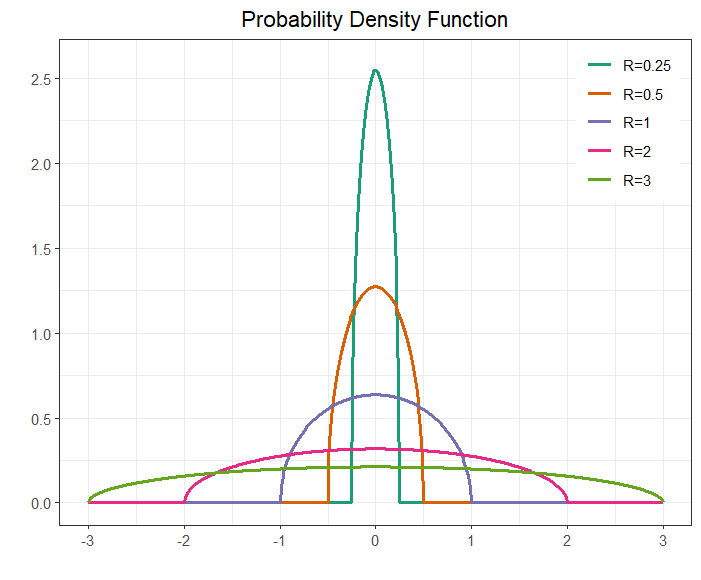
\includegraphics[width=6.5cm,height=6cm]{Figures/PDF_plot.png}
                \end{column}
            \end{columns}
\end{frame}


\subsection{}
\begin{frame}
	\frametitle{Wigner Semicircle Distribution}
        The probability density function is given as:
        \begin{center}
            $f(x)=\frac{2}{\pi R^2}\sqrt{R^2-(x-a)^2}$
        \end{center}
        for $-R \leq x-a \leq R$, and
        \begin{center}
            $f(x)=0$ 
        \end{center}
        if $|x-a|>R$.
\end{frame}


\subsection{}
\begin{frame}
	\frametitle{Wigner Semicircle Distribution - Motivation}
        \begin{center}
            The distribution of the eigenvalues of an N x N i.i.d. random matrix will converge to the semicircle distribution as N goes to infinity.
        \end{center}
\end{frame}


\subsection{}
\begin{frame}
	\frametitle{Random Matrices}
        \begin{itemize}
            \item A random matrix is a matrix in which some or all of its entries are sampled randomly from a probability distribution
            \item An independent and identically distributed (i.i.d.) random matrix is a matrix in which each of its entries is drawn from the same probability distribution
            \item It is important that the matrix is square (N x N)
        \end{itemize}
\end{frame}

    
\begin{frame}[fragile]
  \frametitle{Random Matrices - 5 x 5 Example}
  \begin{lstlisting}
random_matrix_example <- matrix(data = rnorm(25), 5, 5)
  \end{lstlisting}
  \begin{center}
      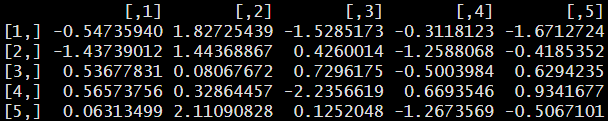
\includegraphics[width=10cm,height=3cm]{Figures/random_matrix_example.png}
  \end{center}
\end{frame}


\subsection{}
\begin{frame}
	\frametitle{Eigenvalues}
        \begin{itemize}
            \item Given:
            \begin{itemize}
                \item An n x n matrix $A$
                \item A non-zero vector $v$ of length n
            \end{itemize}
            \item If $Av$ scales $v$ by a factor of $\lambda$, where $\lambda$ is a scalar, then $v$ is an eigenvector of $A$ and $\lambda$ is the corresponding eigenvalue
            \item The matrix $A$ has at most n eigenvalues
        \end{itemize}
\end{frame}


%%%%%%%%%%%%%%%%%%%%%%%%%
\section{The R Package}  
%%%%%%%%%%%%%%%%%%%%%%%%%


\subsection{}
\begin{frame}
	\frametitle{The R Package: semicircledistr}
        \begin{center}
            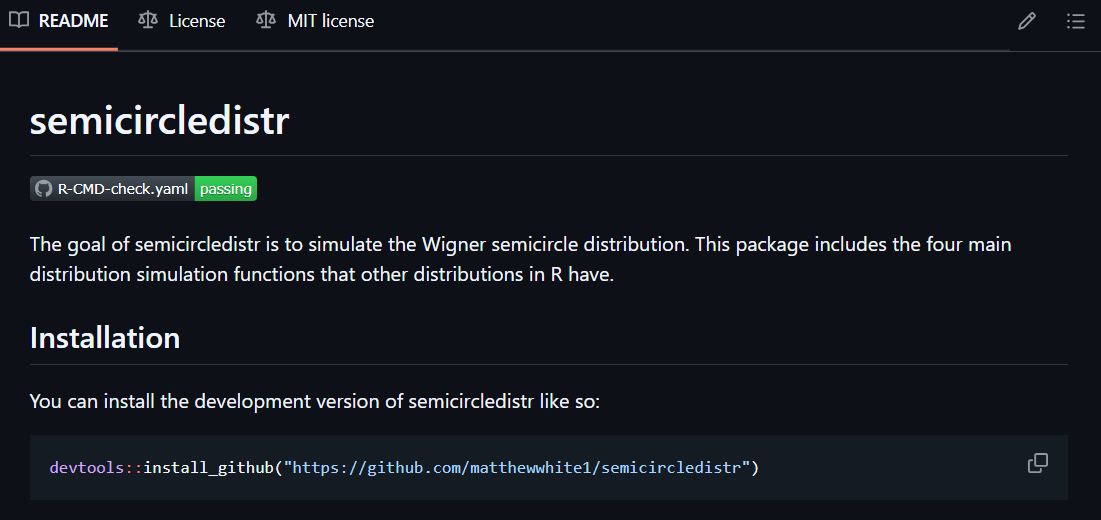
\includegraphics[width=10cm,height=5cm]{Figures/README_top.png}
        \end{center}
\end{frame}


\subsection{}
\begin{frame}
	\frametitle{Semicircle Probability Density Function (PDF)}
            \begin{columns}[T]
                \begin{column}{.4\textwidth}
            	\begin{itemize}
                	\item A PDF is a function whose value is the relative probability that the value of a random variable is equal to that sample
                        \item Implemented as the dsemicircle function
                        \item Allows for an offset parameter, while being centered at 0 is the default
                    \end{itemize}
                \end{column}
                \begin{column}{.6\textwidth}
                    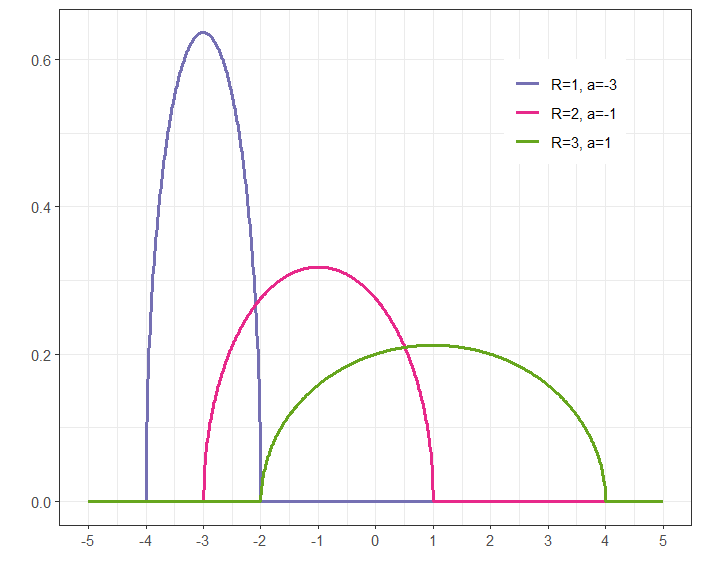
\includegraphics[width=6.5cm,height=6cm]{Figures/PDF_plot_shift.png}
                \end{column}
            \end{columns}
\end{frame}


\subsection{}
\begin{frame}
	\frametitle{Semicircle PDF Implementation}
        \begin{itemize}
            \item Function signature: dsemicirle(x, R, a = 0)
            \begin{itemize}
                \item \textbf{x} is the value to get the PDF of
                \item \textbf{R} is the radius
                \item \textbf{a} is an optional shift parameter
                \item Accepts vectorized input
            \end{itemize}
            \item Performs validation on inputs
            \begin{itemize}
                \item Such as making sure values are numeric
            \end{itemize}
            \item Uses the closed form of the PDF to produce results
            \begin{itemize}
                \item In the range of $[-R+a, R+a]$:
                \begin{center}
                    $f(x)=\frac{2}{\pi R^2}\sqrt{R^2-(x-a)^2}$
                \end{center}
                \item Otherwise, the probability is 0
                \item Closed form obtained from Wikipedia
            \end{itemize}
        \end{itemize}
\end{frame}


\subsection{}
\begin{frame}
	\frametitle{dsemicircle Code}
        \begin{center}
            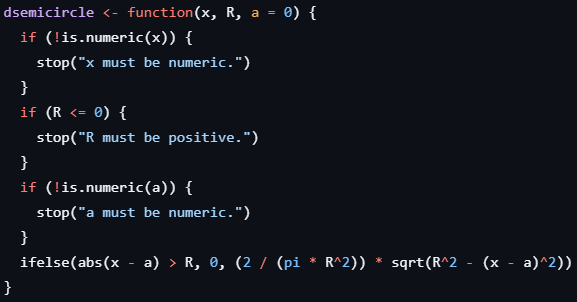
\includegraphics[width=10cm,height=5cm]{Figures/dsemi_code.png}
        \end{center}
\end{frame}


\subsection{}
\begin{frame}
	\frametitle{Semicircle Cumulative Distribution Function (CDF)}
            \begin{columns}[T]
                \begin{column}{.4\textwidth}
            	\begin{itemize}
                	\item The CDF describes the probability that a value is less than or equal to x in the semicircle distribution
                        \item Implemented in the psemicircle function
                    \end{itemize}
                \end{column}
                \begin{column}{.6\textwidth}
                    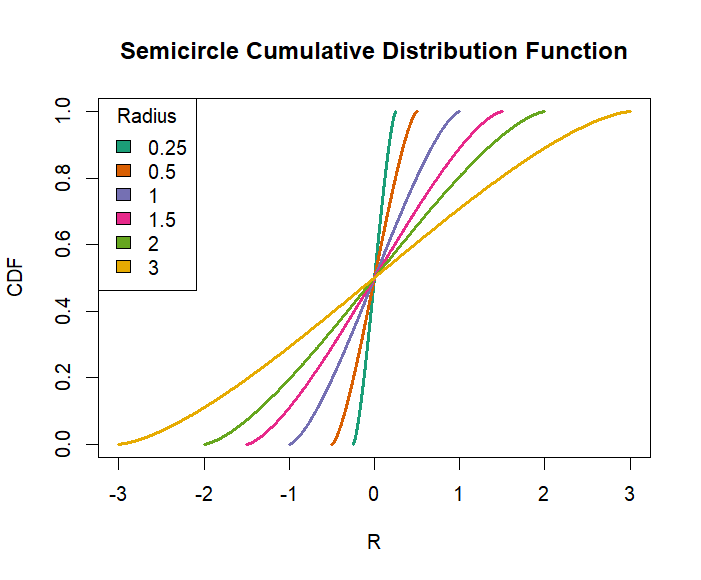
\includegraphics[width=6.5cm,height=6cm]{Figures/CDF_plot.png}
                \end{column}
            \end{columns}
\end{frame}


\subsection{}
\begin{frame}
	\frametitle{Semicircle CDF Implementation (psemicircle)}
        \begin{itemize}
            \item Function signature: psemicirle(x, R, a = 0)
            \begin{itemize}
                \item \textbf{x} is the value to get the CDF of
                \item \textbf{R} is the radius
                \item \textbf{a} is an optional shift parameter
                \item Accepts vectorized input
            \end{itemize}
            \item Performs validation on inputs
            \begin{itemize}
                \item Such as making sure values are numeric and x is within the bounds of the radius
            \end{itemize}
            \item Uses the closed form of the CDF to produce results
            \begin{itemize}
                \item In the range of $[-R+a, R+a]$:
                \begin{center}
                    $\frac{1}{2}+\frac{(x-a)\sqrt{R^2-(x-a)^2}}{\pi R^2}+\frac{\sin^{-1}(\frac{x-a}{R})}{\pi}$
                \end{center}
                \item Closed form obtained from Wikipedia
            \end{itemize}
        \end{itemize}
\end{frame}


\subsection{}
\begin{frame}
	\frametitle{psemicircle Code}
        \begin{center}
            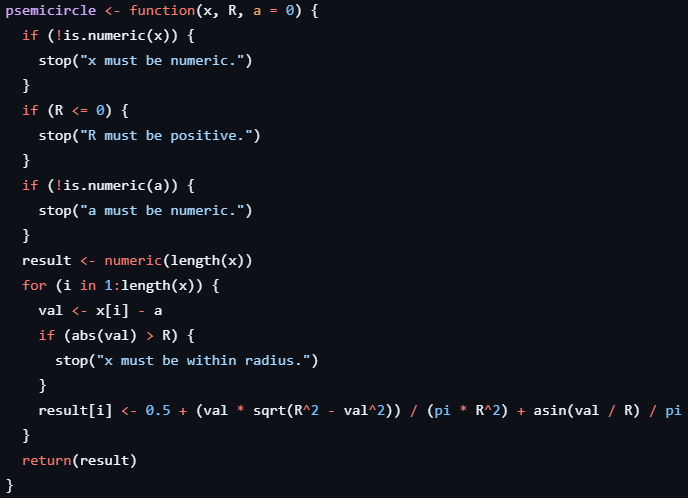
\includegraphics[width=10cm,height=6cm]{Figures/psemi_code.png}
        \end{center}
\end{frame}


\subsection{}
\begin{frame}
	\frametitle{Semicircle Quantile Function Implementation}
        \begin{itemize}
            \item The quantile function is the inverse CDF
            \item There is no closed-form solution
            \item To solve this issue, we used uniroot(), which is a built-in R function solving f(x) = 0
            \begin{itemize}
                \item Finds root (value of x) within an interval such that f(x) is as close to 0 as possible
                \item We solve psemicircle(x, R, a) - p = 0
                \item Finds the quantile \textbf{x} so the cumulative probability up to \textbf{x} equals given \textbf{p}
            \end{itemize}
        \end{itemize}
\end{frame}


\subsection{}
\begin{frame}
	\frametitle{qsemicircle Code}
        \begin{center}
            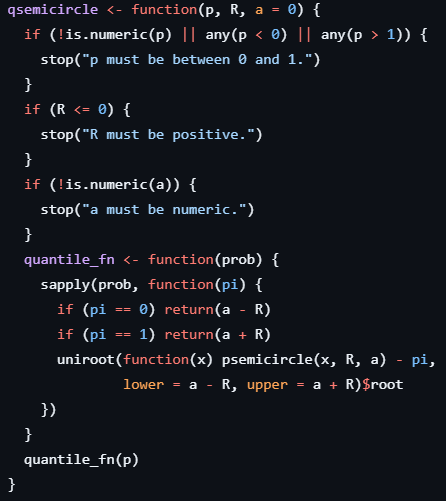
\includegraphics[width=7cm,height=7cm]{Figures/qsemi_code.png}
        \end{center}
\end{frame}


\subsection{}
\begin{frame}
	\frametitle{Random Generation for Value in Distribution (rsemicircle)}
            \begin{columns}[T]
                \begin{column}{.3\textwidth}
            	\begin{itemize}
                	\item Histograms show values generated for different values of R
                    \end{itemize}
                \end{column}
                \begin{column}{.7\textwidth}
                    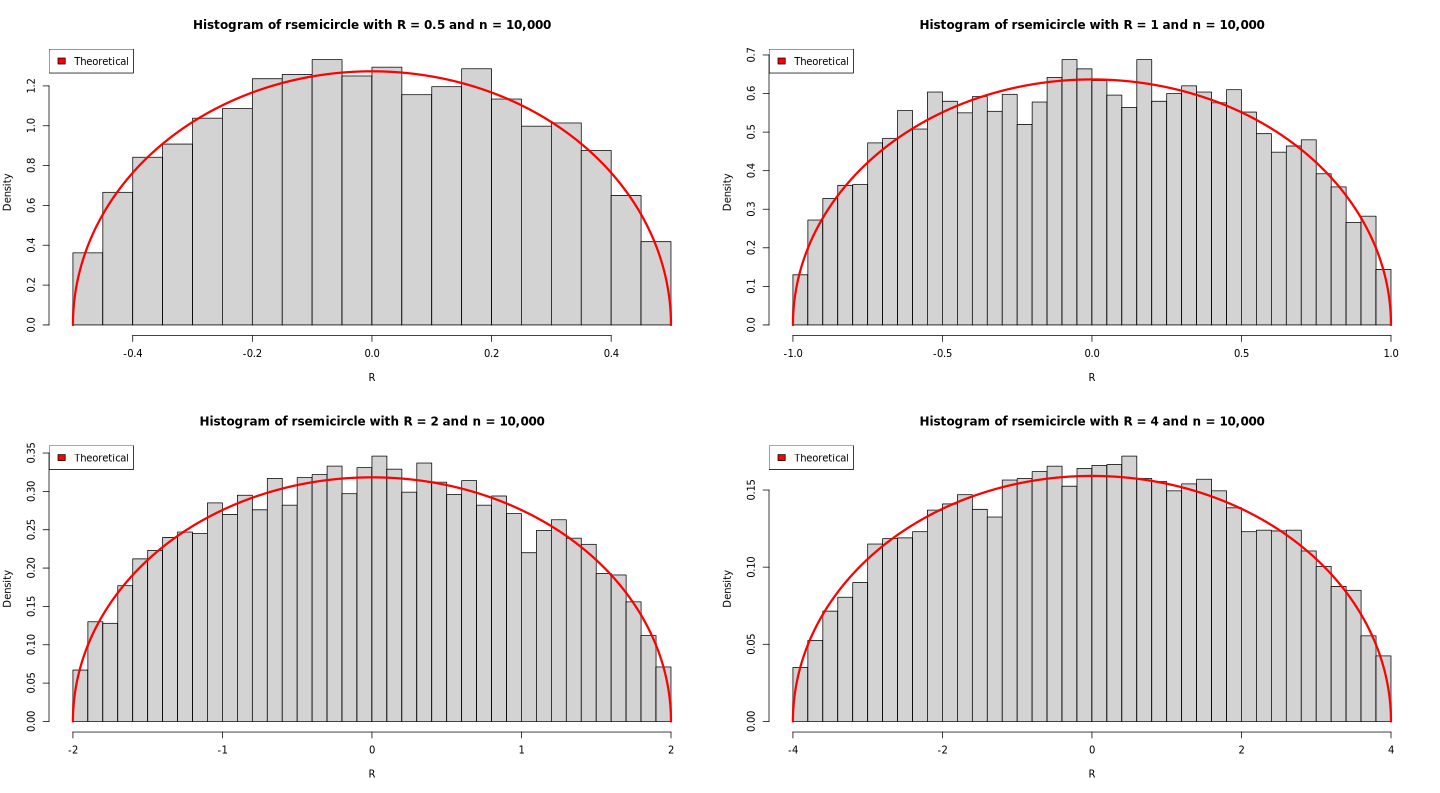
\includegraphics[width=8cm,height=6cm]{Figures/rsemicircle-histograms.png}
                \end{column}
            \end{columns}
\end{frame}


\subsection{}
\begin{frame}
	\frametitle{Semicircle Random Generation Implementation (rsemicircle)}
        \begin{itemize}
            \item Function signature: rsemicirle(n, R, a = 0)
            \begin{itemize}
                \item \textbf{n} is the number of random values to generate
                \item \textbf{R} is the radius
                \item \textbf{a} is an optional shift parameter
            \end{itemize}
            \item Performs validation on inputs
            \begin{itemize}
                \item Such as making sure values are numeric and n is an integer
            \end{itemize}
            \item Leverages the inverse CDF to generate a random value
            \begin{itemize}
                \item The function generates random uniform values from 0 to 1, then passes these values into the inverse CDF function
                \item Uses qsemicircle as the inverse CDF
            \end{itemize}
        \end{itemize}
\end{frame}


\subsection{}
\begin{frame}
	\frametitle{rsemicircle Code}
        \begin{center}
            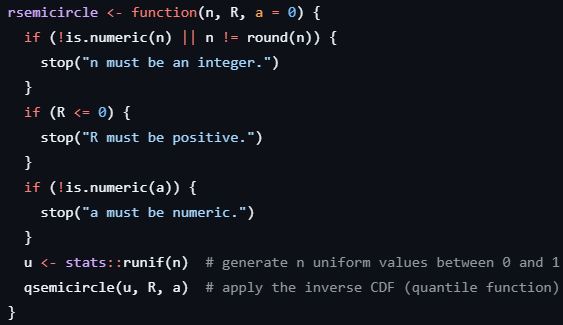
\includegraphics[width=10cm,height=6cm]{Figures/rsemi_code.png}
        \end{center}
\end{frame}


\subsection{}
\begin{frame}
	\frametitle{rsemicircle: Comparison with qsemicircle}
            \begin{columns}[T]
                \begin{column}{.5\textwidth}
            	\begin{itemize}
                	\item If we compare the quantiles of random values generated with rsemicircle with the theoretical quantiles from the distribution generated with qsemicircle we expect to see a straight line
                    \item As shown on the right, the values fall approximately on a straight line
                    \end{itemize}
                \end{column}
                \begin{column}{.5\textwidth}
                    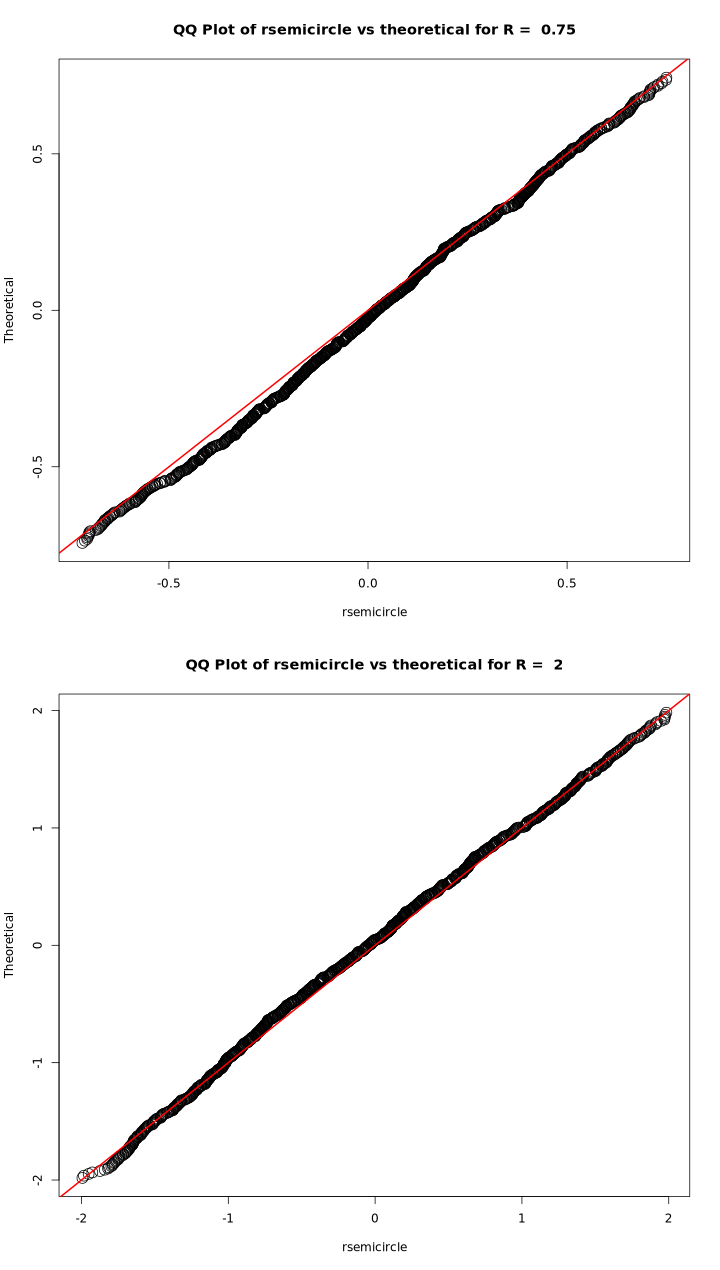
\includegraphics[width=5cm,height=6cm]{Figures/rsemicircle-qq.png}
                \end{column}
            \end{columns}
\end{frame}


\subsection{}
\begin{frame}
	\frametitle{Testing}
        \begin{itemize}
            \item Unit-level testing is performed using the R testthat library
            \item Testing exists for all 4 functions verifying the following:
            \begin{itemize}
                \item The given parameters are of expected type (e.g. the radius is numeric)
                \item The given parameters are within valid range (e.g. x must be within radius for psemicircle)
                \item The functions support vectorization
                \item The functions support the offset parameter (a)
                \item The functions give the expected results for the given inputs, based on theoretical results
            \end{itemize}
            \item Tests are run automatically in GitHub
        \end{itemize}
\end{frame}


\subsection{}
\begin{frame}
	\frametitle{Testing}
        \begin{center}
            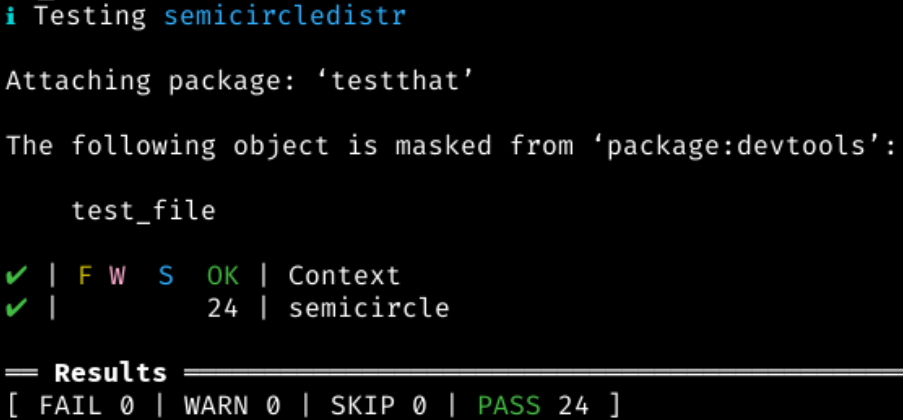
\includegraphics[width=10cm,height=6cm]{Figures/tests.png}
        \end{center}
\end{frame}

%%%%%%%%%%%%%%%%%%%%%%%%%
\section{Applying Package Functions}  
%%%%%%%%%%%%%%%%%%%%%%%%%


\subsection{}
\begin{frame}
	\frametitle{Verification of Wigner's Semicircle Law - Normal Distribution} 
    \begin{itemize}
        \item Recall: The distribution of the eigenvalues of an N x N i.i.d. random matrix will converge to the semicircle distribution as N goes to infinity
        \item Steps to verify this law using R simulation:
        \begin{itemize}
            \item Simulate three Gaussian random matrices with different sizes (1000 x 1000, 2500 x 2500, 5000 by 5000)
            \item Compute the eigenvalues for each matrix
            \item Scale the eigenvalues for easier comparison across histograms - subtract each value in each eigenvalue vector by the mean of the vector and divide by the standard deviation of the vector
        \end{itemize}
        \item After doing this, we found that the range of scaled eigenvalues for each matrix went from -2 to 2
        \item Applying a curve with R = 2 from our dsemicircle function:
    \end{itemize}
\end{frame}


\subsection{}
\begin{frame}
	\frametitle{Verification of Wigner's Semicircle Law - Normal Distribution}
        \begin{center}
            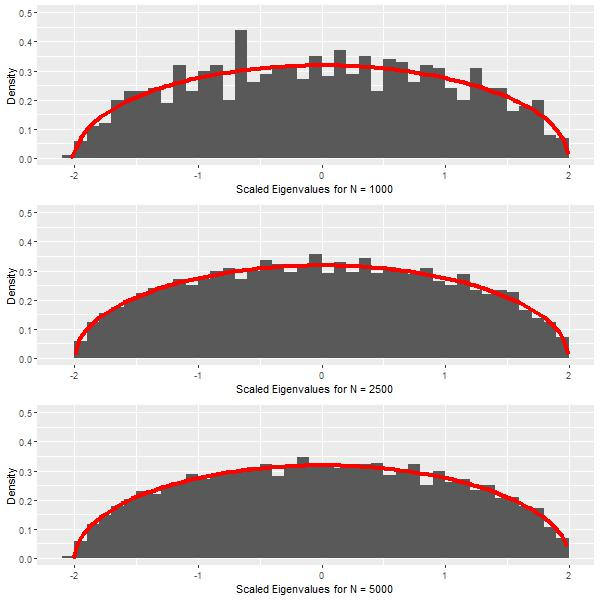
\includegraphics[width=8cm,height=6cm]{Figures/SemiLaw.jpeg}
        \end{center}
\end{frame}


\subsection{}
\begin{frame}
	\frametitle{Verification of Wigner's Semicircle Law - Exponential Distribution}
    \begin{itemize}
        \item As far as we can tell from our online research, Wigner's semicircle law applies to any probability distribution - not just the normal distribution
        \item We followed the same steps on three exponential random matrices with $\lambda=1$
        \item After scaling the eigenvalues, we found that their range was from about -1 to 1, so we chose to apply a curve with R = 0.9:
    \end{itemize}
\end{frame}


\subsection{}
\begin{frame}
	\frametitle{Verification of Wigner's Semicircle Law - Exponential Distribution}
        \begin{center}
            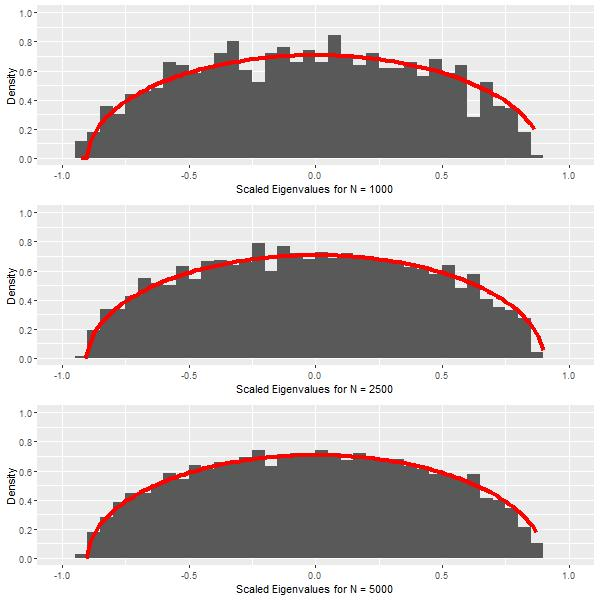
\includegraphics[width=8cm,height=6cm]{Figures/SemiLaw_Exp.jpeg}
        \end{center}
\end{frame}


\subsection{}
\begin{frame}
	\frametitle{Verification of Wigner's Semicircle Law - Uniform Distribution}
    \begin{itemize}
        \item We followed the same steps on three uniform random matrices with a min of 0 and a max of 1
        \item After scaling the eigenvalues, we found that their range was from about -0.6 to 0.6, so we chose to apply a curve with R = 0.55:
    \end{itemize}
\end{frame}


\subsection{}
\begin{frame}
	\frametitle{Verification of Wigner's Semicircle Law - Uniform Distribution}
        \begin{center}
            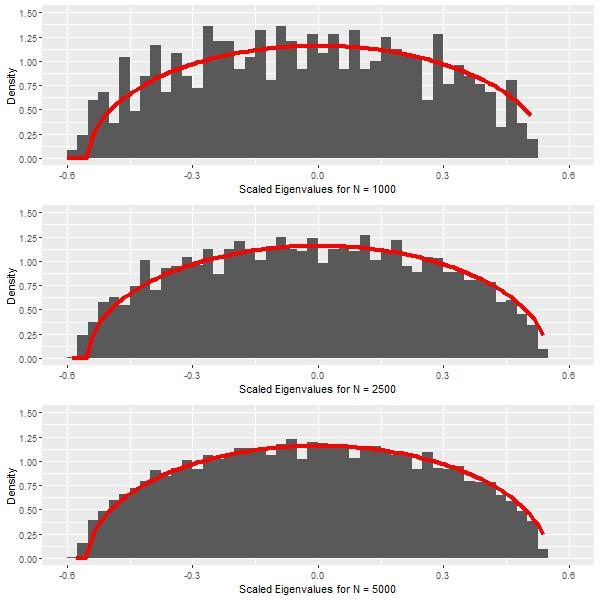
\includegraphics[width=8cm,height=6cm]{Figures/SemiLaw_Unif.jpeg}
        \end{center}
\end{frame}


\subsection{}
\begin{frame}
	\frametitle{Verification of Wigner's Semicircle Law - Semicircle Distribution}
    \begin{itemize}
        \item Finally, we followed the same steps on three semicircle random matrices with a radius of 2
        \item After scaling the eigenvalues, we found that their range was from -2 to 2, so we chose to apply a curve with R = 2:
    \end{itemize}
\end{frame}


\subsection{}
\begin{frame}
	\frametitle{Verification of Wigner's Semicircle Law - Semicircle Distribution}
        \begin{center}
            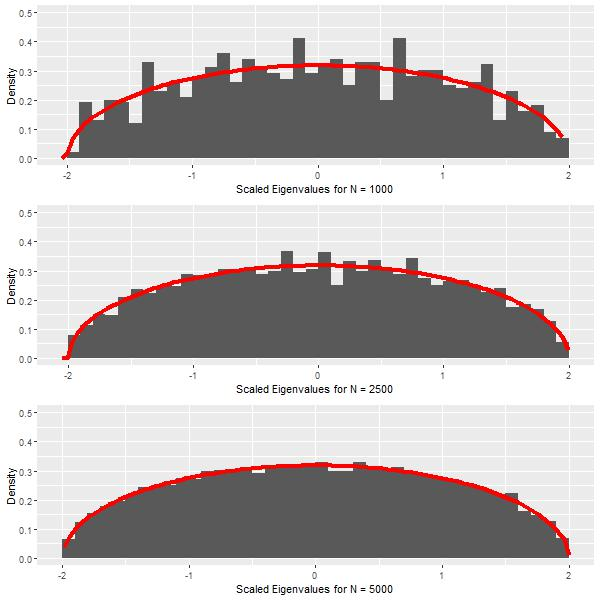
\includegraphics[width=8cm,height=6cm]{Figures/SemiLaw_Semicircle.jpeg}
        \end{center}
\end{frame}


\subsection{}
\begin{frame}
	\frametitle{Verifying a Beta Transformation Theory}
        From Wikipedia:
        \begin{center}
            "If $Y$ is a beta-distributed random variable with parameters $\alpha$ = $\beta$ = $\frac{3}{2}$, then the random variable $2RY-R$ exhibits a Wigner semicircle distribution with radius R."
        \end{center}
\end{frame}


\subsection{}
\begin{frame}
	\frametitle{Verifying a Beta Transformation Theory}
    \begin{itemize}
        \item Steps to verify this theory using R simulation:
        \begin{itemize}
            \item Simulate three random vectors from a Beta distribution with parameters $\alpha$ = $\beta$ = $\frac{3}{2}$ and different sizes (1000, 10000, 100000)
            \item Calculate a transformation of these vectors given $2RY-R$
            \item Examine their distributions
        \end{itemize}
        \item We chose R = 2 to test this theory
        \item Following the above steps output this plot:
    \end{itemize}
\end{frame}


\subsection{}
\begin{frame}
	\frametitle{Verifying a Beta Transformation Theory}
        \begin{center}
            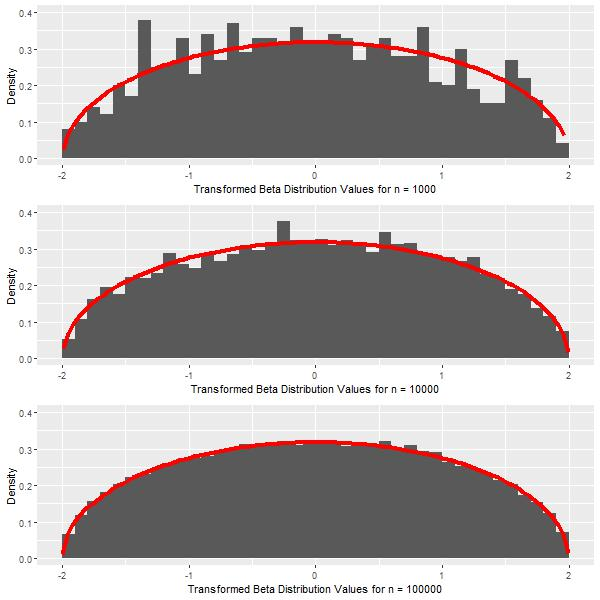
\includegraphics[width=8cm,height=6cm]{Figures/BetaTrans.jpeg}
        \end{center}
\end{frame}


%%%%%%%%%%%%%%%%%%%%%%%%%
\section{Conclusions and Future Work}  
%%%%%%%%%%%%%%%%%%%%%%%%%

\begin{frame}
	\frametitle{Summary}
        \begin{itemize}
            \item We created an R package to simulate the semicircle distribution, which does not have any other current R packages that simulate it
            \item This R package includes the four simulation functions, documentation for these functions, an overall README, and tests
            \item We accomplished everything we said we would in our proposal
            \item If we had more time to work on this project, we would have liked to do some more advanced math with the distribution simulation (calculating moments and conducting some more transforms, some of which are mentioned on Wikipedia)
        \end{itemize}
\end{frame}


\begin{frame}
	\frametitle{Future Work}
        \begin{itemize}
            \item This summer, we will submit this package to CRAN
            \item Before we do this, we still need to:
            \begin{itemize}
                \item Edit the DESCRIPTION file to make it more informative
                \item Select an official package maintainer
            \end{itemize}
            \item Fortunately, we have already completed most of the requirements for having a CRAN-ready R package
            \item Dr. Bean may have some more insight on what we still need to do as the professor currently teaching a course all about R package development
        \end{itemize}
\end{frame}

% References: Syrjala, 4 test aggregations, Chunyang R package; Syrjala applications for eye tracking

\begin{frame}
	\frametitle{References} 
	\scriptsize
	\begin{itemize}
	\item Jiang, T. (2021). {\it Wigner's semicircle law for Gaussian random matrices.} University of Chicago Mathematics REU. \url{https://math.uchicago.edu/~may/REU2021/REUPapers/Jiang,Tianchong.pdf}

	\item Li, L. H. (2020, January 29). {\it Wigner's semicircle law.} MIT Physics Directed Reading Program. \url{https://phys-drp.mit.edu/sites/default/files/lhli_0.pdf}
    
	\item Wikimedia Foundation. {\it Wigner semicircle distribution.} Wikipedia. \url{https://en.wikipedia.org/wiki/Wigner_semicircle_distribution}
	
	\item Wolfram. {\it Wigner's Semicircle Law.} Wolfram MathWorld. \url{https://mathworld.wolfram.com/WignersSemicircleLaw.html}
	
	\end{itemize}
\end{frame}



\end{document}

